\documentclass[12pt]{article}
\usepackage[utf8]{inputenc}
\usepackage{fullpage}
\usepackage{hyperref}
\usepackage{graphicx}
\graphicspath{{./images/}}

\title{Assignment 4: Becoming an Independent Data Scientist Example Solution}
\author{Tom Perneczky}

\begin{document}
	\maketitle
	\section{Region and Domain}
	\textbf{State the region and the domain category that your data sets are about.}\\
	\begin{itemize}
		\item Ann Arbor, Michigan, United States
		\item Weather phenomena
	\end{itemize}
	\section{Research Question}
	\textbf{You must state a question about the domain category and region that you identified as being interesting.}\\
	What is the correlation between the average temperature per month and the average unemployment rate per month over the years 2011-2021 in Ann Arbor?
	\section{Links}
	\textbf{You must provide at least two links to available datasets. These could be links to files such as CSV or Excel files, or links to websites which might have data in tabular form, such as Wikipedia pages.}\\
	\begin{itemize}
		\item \href{https://www.noaa.gov}{https://www.noaa.gov} Weather Data
		\item \href{https://data.bls.gov/timeseries/LAUMT261146000000003?amp%253bdata_tool=XGtable&output_view=data&include_graphs=true}{https://data.bls.gov} Unemployment Data
	\end{itemize}
	\section{Image}
	\textbf{You must upload an image which addresses the research question you stated. In addition to addressing the question, this visual should follow Cairo's principles of truthfulness, functionality, beauty, and insightfulness.}
	\newline
	\newline
	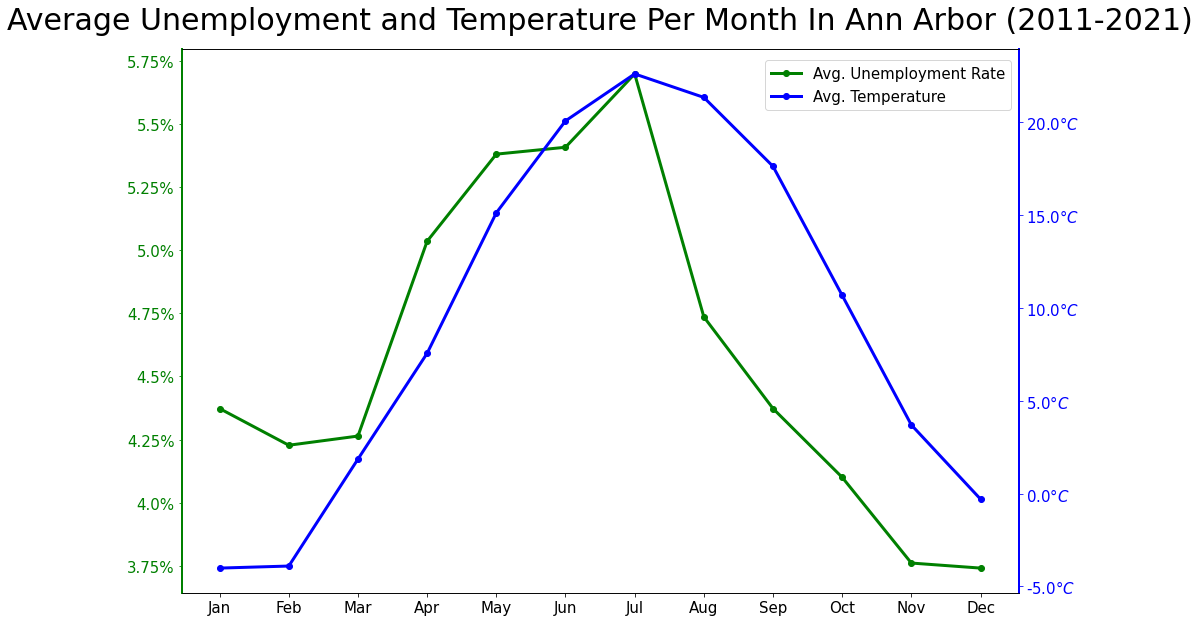
\includegraphics[width=\textwidth]{plot}
	\section{Discussion}
	\textbf{You must contribute a short (1-2 paragraph) written justification of how your visualization addresses your stated research question.}\\
	I plotted the data for temperature and unemployment rate on the same axes so one could see there is definitely a correlation between weather and unemployment in the seasonal context.\\
	Additionally I want to emphasize that both temperature and unemployment rates reach the top in July. According to an \href{https://www.michigan.gov/dtmb/0,5552,7-358--427443--,00.html}{article} of the \href{https://www.michigan.gov}{michigan.gov} website this represents the typical seasonal patterns of Michigan's local labor markets.
	
\end{document}